\section{What worked and what did not}\label{sec:lessons}

\inbrief{Of 141 written hypotheses, 39 were explicitly falsified by pre-set kill
gates. Making the smooth model smoother helped; making it more accurate did not.
Curvature kicks helped about equally along every direction tried, so the record
cannot credit the curvature. A post-competition audit found ten defects; none is
known to have affected the judged entry.}

We ran development as written hypotheses, each with a kill gate (a pre-set threshold
for abandoning the idea) and a recorded outcome: 141 experiments, 39 explicitly
falsified (\historical). \Cref{tab:development} summarizes ten; they are single,
uncontrolled runs, so they show which ideas we kept and why rather than measure
effect sizes. Kill gates and cross-design checks caught a bug (row~3) and a move
that hurt industrial-style designs (row~5). Three lessons recur.

\begin{table}[htbp]
\centering
\footnotesize
\caption{What we tried during development (\historical). Each row summarizes single-run development records from April--May 2026. The runs are uncontrolled: hardware, time budget and concurrency varied, and most comparisons are against a separate reference run. Scores are proxy scores; lower is better. Row 1 gives the September re-measurement (\measurement) in place of the May figure. Verdict records the development decision at the time: \emph{kept}, adopted into a later pipeline; \emph{dropped}, abandoned after a negative result. Appendix~\ref{app:glossary} maps each numbered row to its record.}
\label{tab:development}
\begin{tabularx}{\linewidth}{@{}>{\raggedright\arraybackslash\hsize=0.9\hsize}X>{\raggedright\arraybackslash\hsize=1.1\hsize}Xl@{}}
\toprule
Idea (plain words) & What happened & Verdict \\
\midrule
1.~Rescore only what a one-block move changes, instead of recomputing the whole score & September re-measurement on two designs: 1.3--3.7 ms per move versus 1.4--26.9 s for a full rescore; largest relative difference $2.6\times10^{-15}$. & kept \\
\addlinespace[2pt]
2.~Move one block at a time along one axis to its best legal position; stop when gains level off rather than at a fixed time & Mean over 17 designs 1.1055, versus 1.1193 with a fixed 600 s stop, using 69\% more total time; hard designs gained 1.7--3.6\%, and all 17 stopped before the one-hour cap. & kept \\
\addlinespace[2pt]
3.~After local search stalls, accept some uphill moves at random (simulated annealing) & The first version was worse on 4 of 4 designs (by 5.7\% on average) because it returned its last state rather than its best. Fixed, it gained 0.63\% and became one stage of the earlier serial pipeline. & kept \\
\addlinespace[2pt]
4.~After local search converges, take GPU gradient steps on a smooth approximation of the score to find a better nearby arrangement & 0 of 350 attempts accepted on 4 designs at full budgets; a 2.16\% gain seen with shortened budgets did not reappear. & dropped \\
\addlinespace[2pt]
5.~Choose which blocks to remove and re-place by how much they add to routing congestion & Lower on 2 of 4 IBM designs (by 1.12\% and 0.15\%), but 1.45\% worse on four open industrial-style designs (5.14\% on one) and 0.39\% worse over all 17 IBM designs. & dropped \\
\addlinespace[2pt]
6.~Blend two good but different placements by moving every block partway along a straight line between them & On 2 designs, none of the 9 intermediate blends could be made overlap-free by the 50-iteration repair step; before repair, blends scored up to 61\% worse. & dropped \\
\addlinespace[2pt]
7.~Drive a mature open-source placer's optimizer (DREAMPlace) with the challenge score as its objective & On IBM01, 0.918 after repair and local search versus 0.852 for the existing pipeline (7.7\% worse); the optimizer left 118 overlaps for repair to fix. & dropped \\
\addlinespace[2pt]
8.~Make the smooth routing-congestion model agree more closely with the official scorer & On IBM17 the model's error fell from 14.4\% to 8.0\%, yet the final score was 0.98\% worse; a separate bug fix that also reduced the error changed it by 0.12\%, within noise. & dropped \\
\addlinespace[2pt]
9.~Spread each block's area as a smooth bell-shaped (Gaussian) blur when estimating crowding, so the gradient changes smoothly & Lower on 4 of 4 crowded designs (by 2.71\% on average) than the same pipeline with grid density. A later 17-design run averaged 0.98199, versus 1.05750 for the earlier serial pipeline, lower on 16 of 17. & kept \\
\addlinespace[2pt]
10.~Jointly reassign up to 50 highly connected blocks to candidate slots with an optimal matching (the Hungarian method), then rerun local search & Lower in 5 of 5 single-design trials (0.35--1.25\% against separate reference runs); part of the gain may come from the extra local-search pass. It went into an optional lane that is inferred never to have been scored. & kept \\
\bottomrule
\end{tabularx}
\end{table}


\paragraph{A smoother surrogate helped; a more faithful one did not.} Closer
agreement with the evaluator did not improve final scores (\historical): a
congestion model whose
IBM17 error fell from 14.4\% to 8.0\% left the final score 0.98\% worse (row~8;
within single-design run-to-run spread), and an earlier smooth score that ranked
saved placements well (Spearman 0.929) led descent from a good IBM01 placement to a
result 81\% worse after repair. Gradient polish did not improve converged placements
(rows~4 and~7); the change that helped, Gaussian density (row~9), made the surface
smoother, and its fidelity was not measured.

\paragraph{Good placements can be separated by illegal states.} Straight-line blends
between two good placements were never legal (0 of 9 on two designs; row~6),
consistent with \cref{prop:geometry}, which allows but does not require such gaps.

\paragraph{Curvature kicks helped, but the record cannot credit the curvature.} The
most elaborate idea has the clearest record (\cref{fig:curvature}; \historical). In
v1 research runs without the one-hour cap, a first curvature stage (up to 4,007\,s
per design) lowered the mean \emph{plateau} score, the better of v1's two branches
before any kick, from 1.08128 to 1.06760, and a cascade of further stages (up to
3,454\,s) reached 1.06119. Every design improved, but no design could have gotten
worse: a stage keeps its input unless a candidate scores lower. The informative
evidence is which kicks worked, and success barely depends on the eigenvector or the
step length. Of 204 first-stage attempts (12 on each design), 201 could be legalized
and 190 ended below the plateau with zero overlap: 94 of 102 along the first
eigenvector, 96 of 102 along the second, and 64, 65 and 61 of 68 at total
displacement norms of 0.3, 1 and 3\,$\mu$m summed over all blocks. Generic
perturb-and-repolish, or the extra polish alone, would produce this pattern; the
missing experiments are a random-direction control and a zero-step (polish-only)
control of equal cost.

\begin{figure}[tbp]
\centering
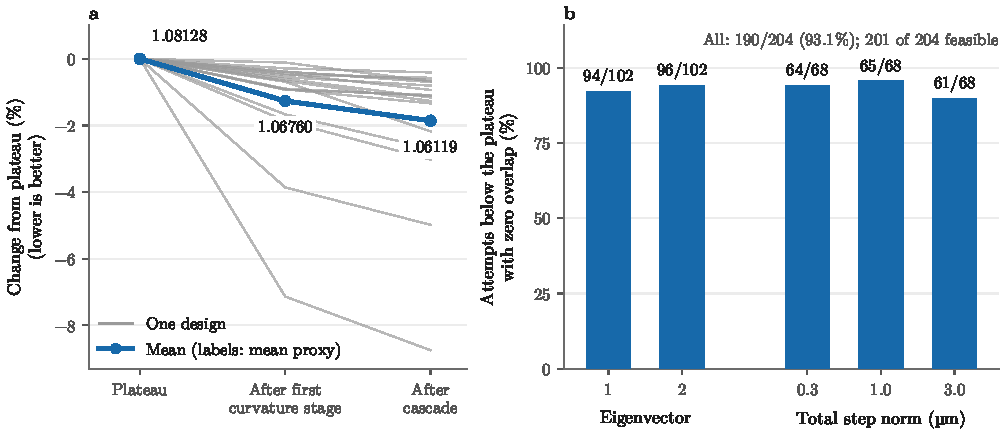
\includegraphics{figures/curvature_attempts.pdf}
\caption{Curvature kicks (perturb along a computed negative-curvature direction, then
legalize and re-polish) in v1 research runs without the one-hour cap (\historical):
(a)~score change relative to the plateau, the best v1 result before any kick, per
design and on average; (b)~share of first-stage attempts ending below the plateau
with zero overlap, by eigenvector and step length. Success is nearly the same in
every group, as generic perturb-and-repolish or the extra polish alone would also
produce.}
\label{fig:curvature}
\end{figure}

The curvature itself is doubtful. At one saved IBM01 placement, automatic
differentiation reports a negative curvature of $-0.442458$, but that number
describes only the smooth branch of the surrogate the point happens to sit on.
Density and congestion branch boundaries lie within $10^{-7}\,\mu$m, so a direct
finite-difference check sees jumps in the gradient instead; on the smooth wirelength
term the two agree to about $4\times10^{-9}$. The surrogate has no true second
derivative there: its eigenvectors are reasonable candidate directions, not
measurements of a bend in the score (\measurement; Appendix~\ref{app:curvature}).

\paragraph{Assignment.} Hungarian reassignment lowered the score in all 5
single-design trials (0.35--1.25\%; row~10), partly perhaps through its extra polish,
and went into Lane~C (\cref{sec:scored}).

\paragraph{Post-competition audit.} A September audit of the competition code found
ten defects, all since repaired (Appendix~\ref{app:verification}). Most were in
parts that were never scored, such as the three-lane supervisor, which waited
without a deadline once its budget had passed and saved lane results only on normal
completion, or in input parsing for hierarchical designs, which the flat IBM designs
never exercise; on all 17 IBM designs the repaired parsing yields identical inputs
(\measurement). Two could touch the single pipeline and cannot be excluded, because
no judged coordinates survive: float32 export can round a coordinate one step past
the upper canvas edge, and input soft clusters outside the canvas, present in 15 of
the 17 IBM inputs, were not explicitly repaired. The organizers' verification passed
the entry.
